\documentclass[letterpaper, 10 pt, conference]{ieeeconf}  % Comment this line out if you need a4paper

%\documentclass[a4paper, 10pt, conference]{ieeeconf}      % Use this line for a4 paper

%\IEEEoverridecommandlockouts                              % This command is only needed if 
                                                          % you want to use the \thanks command

%\overrideIEEEmargins                                      % Needed to meet printer requirements.

% See the \addtolength command later in the file to balance the column lengths
% on the last page of the document

% The following packages can be found on http:\\www.ctan.org
\usepackage{graphics} % for pdf, bitmapped graphics files
\usepackage{epsfig} % for postscript graphics files
\usepackage{graphicx}
\usepackage{mathptmx} % assumes new font selection scheme installed
\usepackage{times} % assumes new font selection scheme installed
\usepackage{mathtools} % assumes amsmath package installed
\usepackage{amssymb}  % assumes amsmath package installed
\usepackage{tikz}
\usepackage{tabulary}
\newcommand{\hvec}{\overset{\rightharpoonup}}
\newcommand{\argmin}{\arg\!\min}
\newcommand{\norm}[1]{\left\lVert#1\right\rVert}
\newcommand{\quotes}[1]{``#1''}
\usetikzlibrary{calc,positioning, fit, arrows}
%\usepackage{biber}

%for citing webcites
\usepackage{cite}
\usepackage{url}

\makeatletter
\newenvironment{tablehere}
  {\def\@captype{table}}
  {}

\newenvironment{figurehere}
  {\def\@captype{figure}}
  {}
\makeatother

\newcommand{\vect}[1]{\ensuremath{\mathbf{#1}}}
\newcommand{\mat}[1]{\ensuremath{\mathbf{#1}}}
\newcommand{\transpose}{\ensuremath{\mathsf{T}}}
\newcommand{\of}[1]{\ensuremath{\left(#1\right)}}

\title{\LARGE \bf
Multi-dimensional Optimization of Gasoline-fueled Variable Pitch Multirotor Aircraft
}


\author{Dallin Briggs, Gary Ellingson% <-this % stops a space
%\thanks{$^{1}$James Jackson is a MS student in the Department of Mechanical Engineering, Brigham Young University
%        {\tt\small jamesjackson@byu.edu}}%
%\thanks{$^{2}$Gary Ellingson is a MS student in the Department of Mechanical Engineering, Brigham Young University
%        {\tt\small gary.ellingson@byu.edu}}%
}


\begin{document}



\maketitle
\thispagestyle{empty}
\pagestyle{empty}


%%%%%%%%%%%%%%%%%%%%%%%%%%%%%%%%%%%%%%%%%%%%%%%%%%%%%%%%%%%%%%%%%%%%%%%%%%%%%%%%
\begin{abstract}

Currently, there are numerous multirotor UAVs that are available commercially and to consumers that are capable of lifting small payloads for an endurance of approximately 30 minutes. While these current multirotors are good for short endurance missions, there are few options for larger, higher payload capacity multirotors that are able to maintain flight for longer than an hour. This paper describes the optimization process used to develop a multirotor platform that maximizes the flight time of a gasoline-fueled multirotor UAV by varying several design variables related to the power required and the aerodynamics of the model.

\end{abstract}


%%%%%%%%%%%%%%%%%%%%%%%%%%%%%%%%%%%%%%%%%%%%%%%%%%%%%%%%%%%%%%%%%%%%%%%%%%%%%%%%
\section{INTRODUCTION}

The creation of a multirotor aircaft capable of both carrying a relatively large payload and flying for a long duration would be very desirable fo many applications.

Designing a gas powered multirotor aircraft requires several design decisions. When considering the total flight time of a the aircraft, foremost of these design decisions are the choice of rotor, engine and gas tank size.  These, and other, trade-offs are hard for a designer to simultaneously consider. 

This paper presents analysis and optimization methods for designing a gas powered multirotor aircraft.  The analysis focuses on modeling the engine and aerodynamic components with a limited consideration of aircraft structure.  These analyses are then used within multi-dimensional optimization to produce a vehicle design capable of long duration flight. 

%%%%%%%%%%%%%%%%%%%%%%%%%%%%%%%%%%%%%%%%%%%%%%%%%%%%%%%%%%%%%%%%%%%%%%%%%%%%%%%
\section{Background}

Multirotor aircraft are useful for a variety of applications.  Because multirotors aircraft can fly vertically they do not required landing strips.  They can carry sensor equipment for scientific or surveillance purposes. Multirotor use in package delivery is being studied by several large companies such as Google, Amazon and DHL \cite{Amazon2014}.   

Incorporating a gas powered engine into a multirotor requires more then just exchanging the electric motors and batteries for an engine and a gas tank respectively. The control of such a vehicle would also fundamentally change.  Electric multirotors are controlled by varying propeller rotational speed to produce varying thrust and torque. Gas engines lack the ability to vary speed quickly enough to control the attitude of a multirotor aircraft. This means a fixed speed and variable pitch propeller is better suited for a gas powered vehicle.

Control of variable pitch multirotor aircraft was studied by Cutler \cite{Cutler2012}. There is a small, electric variable pitch quad commercially available \cite{stingray2016}.  There are also several hobbyist attempts at gas powered variable pitch quads \cite{diy2016}, \cite{hackaday2016}.

In our knowledge there has been no attempt to use a gas powered variable pitch quad to maximize the flight time for carrying a relatively large payload. 

There are many commercially available parts for a gas quad, including engines \cite{da2016} and variable pitch helicopter propellers \cite{align2016}. However, a gas powered multirotor would required a custom frame for mounting the engine and supplying power from the engine to the individual rotors.

FAA requirements \cite{faa2016} specify that model aircraft must weigh less then 55 lbs (25 kg) or else they require special airworthiness certificates.

\section{MOTIVATION}

Nearly all commercial and consumer multirotor UAVs are powered by lithium-polymer batteries because of their high energy capacity to weight ratios. Although these batteries are very useful and reliable, they still offer much lower specific energy ratios then that of liquid fuels such as gasoline. The average specific energy for lithium-polymer batteries is up to 0.95 MJ/kg, where gasoline is 46.4 MJ/kg. This means that a gasoline-fueled multirotor can potentially fly much longer than a battery powered vehicle because it can carry more energy.  

The gass powered quadcopter will have variable pitch propellers would be  
\begin{itemize}
	\item{Will talk more about some of the details using a gas engine entails in the paper.}
	\item{Speak briefly on the reasons for requiring variable pitch with a gas engine.} 
	\item{Speak on current platforms and capabilities and explain how this could fundamentally change the way multirotors are used in commercial applications, but not really for consumers.}
\end{itemize}


\begin{figurehere}
	\begin{center}
		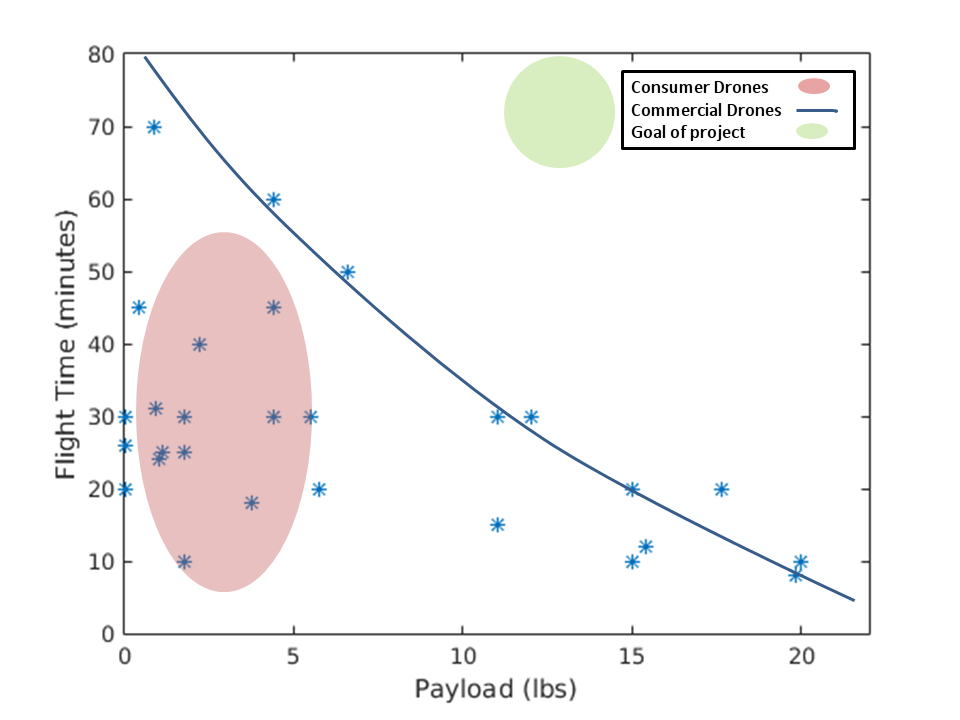
\includegraphics[width=.40\textwidth]{current_capabilities.png}
		\caption{\textit{Graphic showing current platforms and how our would be better.}}
		\label{current_cap}
	\end{center}
\end{figurehere}

	
%%%%%%%%%%%%%%%%%%%%%%%%%%%%%%%%%%%%%%%%%%%%%%%%%%%%%%%%%%%%%%%%%%%%%%%%%%%%%%%%%%
\section{METHODS}

Because the quad is going to be build using commercially available off-the-shelf parts the optimization must be closely based on reality.  The analysis must, therefore, either be based on observations from available hardware or attempt analyze the hardware in its available configuration.  The following sections present some surrogate models for approximating engine parameters as well as aerodynamic analysis of common variable pitch RC propellers. 

\subsection{Engine} 

The designer essentially can only choose the size of engine. All the other data about the engine (mass, maximum power, etc.) have to be a function of displacement size.  Data was collected for popular two stroke RC aircraft engines from several sources to produce the models for other unknown parameters. One source was Desert Aircraft \cite{da2016}.  Figure~\ref{fig:mass} shows the collected data for engine size and mass.  We performed a linear least squares bast fit to produce a model for use in our analysis.

\begin{figure}
	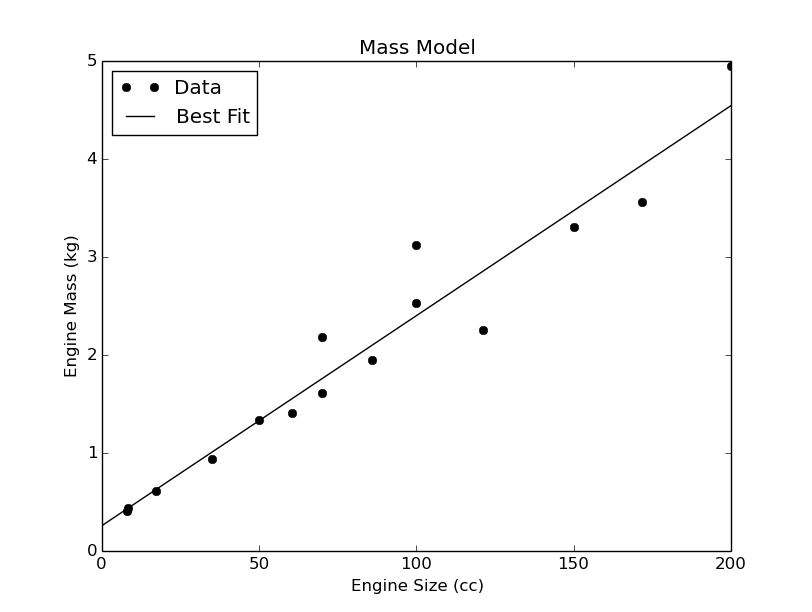
\includegraphics[width=0.5\textwidth]{mass.png}
	\caption{The empirical based surrogate model of engine mass as a function of displacement size. Data from desertaircraft.com \cite{da2016}. $\ y = ax + b \quad a = 0.02145 \quad b = 0.25412$}
		\label{fig:mass}
\end{figure}

Data was also used to produce a model of the power output of the engine as a function of size. Figure~\ref{fig:power} shows that collected data for engine size and power.  Again we initially used a linear least squares fit to the data as well as compared our fit to data produced by Barnard Microsystems \cite{barnardmiro2016}. However both models were inadequate for our analysis because they contain a non-zero y-intercept.  A non-zero y-intercept would allow an infinitely small engine to produce power and thus would allow the aircraft to fly infinitely. To fix this deficiency we applied a quadratic fit to the data and forced it to do through the origin.

\begin{figure}
	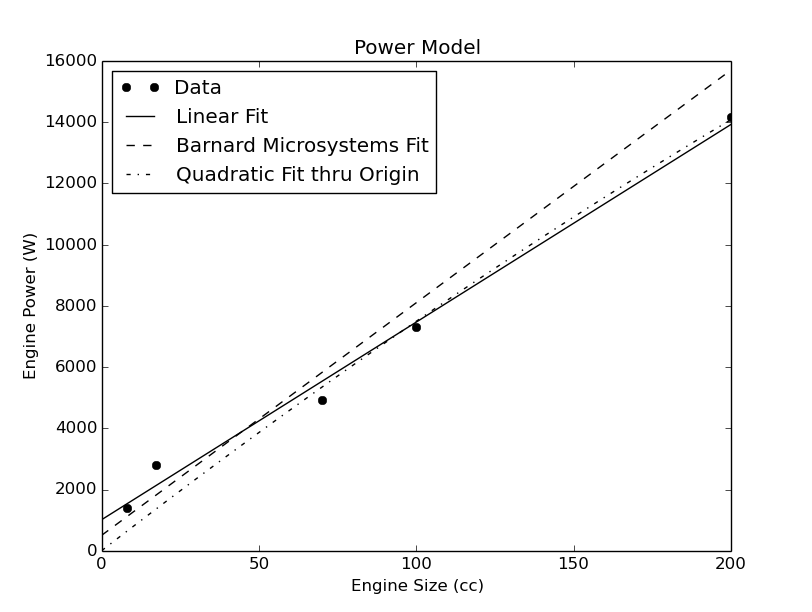
\includegraphics[width=0.5\textwidth]{max_power.png}
	\caption{Empirical based surrogate model of engine maximum power as a function of displacement size. Notice the linear models have a non-zero y intercept but the quadratic fit goes through the origin. Data from desertaircraft.com \cite{da2016} and barnardmicrosystems.com \cite{barnardmiro2016} $\ y = ax^2 + bx \quad a = -0.04548 \quad b = 79.504$}
		\label{fig:power}
\end{figure}


The engine efficiency was not modeled for this project and was assumed a constant parameter.  Within the analysis the shaft output power of the engine was 15\% of the power consumed from the fuel.  

\subsection{Aerodynamics}

Much of the work done in the methodology of optimizing flight time was to find adequate models for the thrust, torque, and power required from the main rotor disks. Since each rotor will be designed using small-scale helicopter components that consist of variable-pitch rotors that have no twist, a simplified helicopter rotor aerodynamic model should be sufficient for these calculations. 

Many of the existing aerodynamic models used in the aerospace industry to represent helicopter rotors are extremely complex and require specialized software tools (many of which are proprietary). High fidelity aerodynamic models generally require lots of computational power; so in order to focus on optimization methods rather than the complex aerodynamics of the system, several simplifications were made.

Combined differential blade element and momentum theory for nonuniform inflow was used to calculate the thrust and the torque differentially across each rotor blade \cite{bramwell2001bramwell}. Using blade element theory, the differential thrust is given by

\begin{equation}
	dT_{prod} = \frac{1}{2} \rho a \Omega^2 r^2 (\theta - \phi) c \  dr,
	\label{thrust_eqn}
\end{equation}

where $\rho$ is the air density, \textit{a} is the lift-curve slope for the blade airfoil, $\Omega$ is the angular velocity of the rotors, \textit{r} is the radius of the annulus of the rotor being differentiated, $\theta$ is the blade pitch angle measured from the horizontal plane formed by the rotational disc of rotor blades, \textit{c} is the chord of the rotor, and $\phi = \tan^{-1}(U_p/U_T) $ is the inflow angle at the blade element. $U_P$ and $U_T$ are the components of air velocity relative to blade element perpendicular and tangential to the plane of rotation, respectively. The total thrust on each rotor is calculated by integrating equation \ref{thrust_eqn} across the rotor radius, \textit{R}. The total thrust for the multirotor, $T_{prod}$ can then be calculated by multiplying the blade thrust by the number of \textit{N} rotors. 

The differential torque for each rotor blade is given by

\begin{equation}
	dQ_{req} = \frac{1}{2} \rho \Omega^2 r^3 c (\delta + \phi C_L) \ dr,
	\label{torque_eqn}
\end{equation}

where $\delta$ is the local blade drag coefficient, and $C_L$ is the lift coefficient. The total torque for the multirotor , $Q_{req}$, can be found using the same method for calculating the thrust. 

The differential power produced by each rotor is then given by 

\begin{equation}
	dP_{req} = dQ\Omega,
	\label{power_eqn}
\end{equation}

and the total power required by the rotors, $P_{req}$, can be calculated using the same method as thrust and torque. 

Equations \ref{thrust_eqn}, \ref{torque_eqn} and \ref{power_eqn} are used in the constraints, as discussed in the Optimization section. In practice, the thrust, torque, and power were integrated in a \textit{for loop} that divided each blade into 10 elements and then summed the differential values for each element. More divisions were made, but it greatly increased the computation time of the optimization algorithm and the results were approximately the same. 

Since the goal of this project is to optimize the flight time of a multirotor and then build it using existing remote controlled aircraft components, a NACA 0012 airfoil was used in the analysis for calculating the coefficient of lift, $C_L$, and the blade element drag coefficient, $\delta$. Data points for this airfoil were generated using Xfoil. This data was then fit with polynomials to approximately represent $C_L$ and $\delta$ across the range of the angle of attack, $\alpha$, continuously, where $\alpha = \theta - \phi$. 

Momentum theory allows for a relatively simple calculation of the inflow angle for each element of the blade. This calculation is an approximation, but it is sufficient for our lower fidelity model in designing the rotor system. The inflow angle is given by 

\begin{equation}
\phi^2 = (\frac{a\sigma}{8})(\theta-\phi),
\label{inflow_eqn}
\end{equation}

where 

$$\sigma = \frac{bc}{\pi r}$$

is the blade solidity ratio based on local rotor radius, and \textit{b} is the number of blades in each ratio. 


\section{OPTIMIZATION}

Our design variables are rotor radius, fuel consumption rate, number of blades per rotor, number of rotors, rotor speed, rotor pitch, engine size, and fuel capacity. Rotor radius and number of blades per rotor, and number of rotors were chosen because this is an easy parameter to vary on multirotors due to the availability of numerous rotor blades available for small rotor aircraft. These variables also have a large influence on the flight time of the multirotor. Rotor speed and rotor pitch were chosen because these variables are easy to change on the physical system through selecting the proper gearing ratios. Fuel consumption rate seems like an odd variable for an optimizer because intuitively an optimizer would just minimize this value to maximize the flight time; however, fuel consumption rate is constrained by the size of engine required to produce the amount of power needed to provide enough lift for the multirotor. All of these design variables, however, have bound constraints that keep them in a reasonable space of commercially available parts/performance.

Setup the formal optimization problem
\begin{equation}
min. \quad f\of{x} = -t_{flight}\of{x}
\label{eq:objective}
\end{equation}
\begin{equation}
w.r.t. \quad x = [variables]^T
\label{eq:vars}
\end{equation}
\begin{equation}
s.t. \quad cons\of{x} \leq 0 
\label{eq:constrants}
\end{equation}

Flight time was calculated by 
\begin{equation}
	t_{flight} = K_{energy}*f_{capacity}/f_{rate}.
\end{equation}
Without constraints, the solution to maximizing flight time would be trivial to calculate as well as impossible to construct. Therefore to optimize the system we must use constraints that ensure the quad is feasible. The constrains are on the power produced by the engine ($P_{prod}$), power required by the prop ($P_{req}$), thrust produced by the prop ($T_{prod}$), lift required by the quad ($T_{req}$) and maximum power capabilities of the engine ($P_{max}$). Where $P_{preq} \leq P_{prod}$, $T_{req} \leq T_{prod}$, and $P_{prod} \leq P_{max}$.

We then will discuss the following:
\begin{itemize}
	\item{scaling of the design variables}
	\item{how we got gradients}
	\item{the optimization method that we utilized}
	\item{python vs matlab benefits and challenges}
\end{itemize}

Since we can only optimize for maximum flight time give a payload (parameter) we can further explore how the characteristics of a gas quad change as we optimize the flight time for different payloads. It may turn out that the optimal quad parameters change greatly as it is optimized for different payload.  In this case we could choose several payloads and optimize over all of then together. \textit{We will present these results with a figure and some discussion.}

\begin{figurehere}
	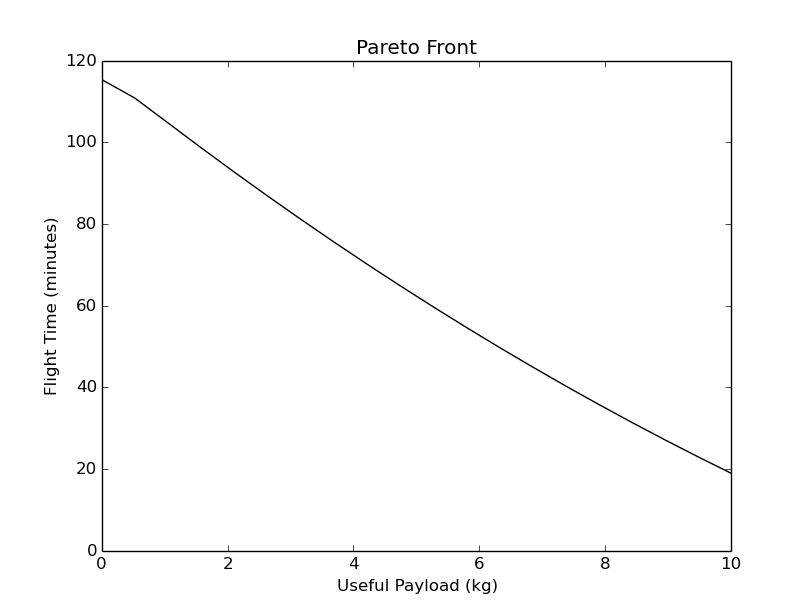
\includegraphics[width=0.5\textwidth]{pareto_front.png}
	\caption{Stand in figure showing optimal flight time as a function of payload.}
		\label{fig:payload}
\end{figurehere}

%Here we can do some discussion on constraint sensitivity - aerodynamics, engine efficiencies...

\section{RESULTS AND DISCUSSION}

We have found that if the design variables are left unbound and all of the constraints are still being met, the maximum flight time could be 11.32 hours. The values of these design variables can be seen in table \ref{table:unbound_results}. 

\begin{tablehere}
\centering
\begin{tabulary}{0.5\textwidth}{|C|C|C|C|C|}
\hline
  \# of Blades & Rotor Radius & Rotor Speed & \# of Rotors \\ \hline
  3 & 2.306 & 39 & 8 \\ \hline
  Blade Pitch & Fuel Rate & Engine Size & Fuel Capacity \\ \hline
  22 & 2.01e-4 & 11.31 & 12.77 \\ \hline
\end{tabulary}
\caption{Optimal design variables for loosely bound constraints. Rotor radius is in meters, rotor speed is in RPM, blade pitch is in degrees, fuel rate is in kg/s, engine size is in cc, fuel capacity is in liters.}
\label{table:unbound_results}
\end{tablehere}



%%%%%%%%%%%%%%%%%%%%%%%%%%%%%%%%%%%%%%%%%%%%%%%%%%%%%%%%%%%%%%%%%%%%%%%%%%%%%%%%%%

\section{CONCLUSION}

lots of really good conclusions

%%%%%%%%%%%%%%%%%%%%%%%%%%%%%%%%%%%%%%%%%%%%%%%%%%%%%%%%%%%%%%%%%%%%%%%%%%%%%%%%
% \section*{APPENDIX}

% Appendixes should appear before the acknowledgment.

% \section*{ACKNOWLEDGMENT}

% Important people/organizations who made it possible


%%%%%%%%%%%%%%%%%%%%%%%%%%%%%%%%%%%%%%%%%%%%%%%%%%%%%%%%%%%%%%%%%%%%%%%%%%%%%%%%

\bibliography{./library}
\bibliographystyle{ieeetr}



\end{document}


%%%%%%%%%%%%%%%%%%%%%%%%%%%%%%%%%%%%%%%%%%%%%%%%%%%%%%%%%%%%%%%%%%%%%%%%%%%%%

% SAVED STUFF






%new document




